\documentclass[__main__.tex]{subfiles}

\begin{document}

\textbf{Электрический диполь} — идеализированная электронейтральная система, состоящая из точечных и равных по абсолютной величине положительного и отрицательного электрических зарядов.

Другими словами, электрический диполь представляет собой совокупность двух равных по абсолютной величине разноимённых точечных зарядов, находящихся на некотором расстоянии друг от друга

Произведение вектора $ \vec l$, проведённого от отрицательного заряда к положительному, на абсолютную величину зарядов $ q\,,$ называется дипольным моментом: $\vec d=q\vec l$.

Во внешнем электрическом поле $\vec E$ на электрический диполь действует момент сил ${\vec d}\times{\vec E}$, который стремится повернуть его так, чтобы дипольный момент развернулся вдоль направления поля.

Потенциальная энергия электрического диполя в (постоянном) электрическом поле равна $-{\vec E}\cdot{\vec d}$. (В случае неоднородного поля это означает зависимость не только от момента диполя - его величины и направления, но и от места, точки нахождения диполя).

Вдали от электрического диполя напряжённость его электрического поля убывает с расстоянием $R$ как $R^{-3}$, то есть быстрее, чем у точечного заряда ( $E \sim R^{-2}$).

Любая в целом электронейтральная система, содержащая электрические заряды, в некотором приближении (то есть собственно в дипольном приближении) может рассматриваться как электрический диполь с моментом $\vec d = \sum_i q_i {\vec r}_i$, где $q_{i}$ — заряд $i$-го элемента, ${\vec r}_i$ — его радиус-вектор. При этом дипольное приближение будет корректным, если расстояние, на котором изучается электрическое поле системы, велико по сравнению с её характерными размерами.
\\
Найдём \textbf{потенциальную энергию}, которой обладает диполь во внешнем электрическом поле (см. Рисунок 1). Эта энергия будет равна:

\begin{equation}
\textit{П} = q\varphi_+ - q\varphi_- = q(\varphi_+ - \varphi_-),
\end{equation}

где $\varphi_+$ и $\varphi_-$ - значения потенциалов внегнего поля в точках, где находятся заряды $+q$ и $-q$.

\begin{equation}
\varphi_+ - \varphi_- = \frac{d\varphi}{dx} \Delta x = \frac{d\varphi}{dx} l \cos \alpha.
\end{equation}

\begin{center}
	
	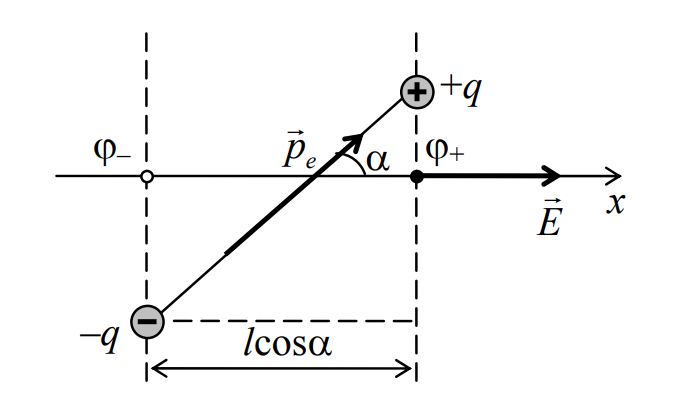
\includegraphics[]{e01_1.png}
	
	Рисунок 1
	
\end{center}

Подставив выражение (0.2) в (0.1) и учитывая, что $E = -\frac{d\varphi}{dx}$, получим:

\begin{equation}
\textit{П} = q\frac{d\varphi}{dx} l \cos \alpha = -qEl\cos \alpha = -p_e E \cos \alpha
\end{equation}

Так как угол $\alpha$ в формуле (0.3) - это угол между векторами $\vec{E}$ и $\vec{p_e}$, то данное выражение можно записать в виде:

\begin{equation}
\textit{П} = - \vec{p_e} \vec{E}
\end{equation}

Выражение (0.4) не учитывает энергию взаимодействия зарядов $+q$ и $-q$, образующих диполь.

Рассмотрим поведение диполя во внешнем электрическом поле. Если диполь поместить в однородное электрическое поле, образующие диполь заряды $+q$ и $-q$ окажутся под дейстивем равных по величине, но противоположных по направлению сил $\vec{F_1}$ и $\vec{F_2}$ (см. Рисунок 2).
Момент пары сил, действующих на диполь, будет равен:

\begin{equation}
M = Fd = Fl\sin \alpha = qEl\sin \alpha = p_e E \sin \alpha,
\end{equation}
где $d = l\sin \alpha$ - момент пары сил.

\begin{center}
	
	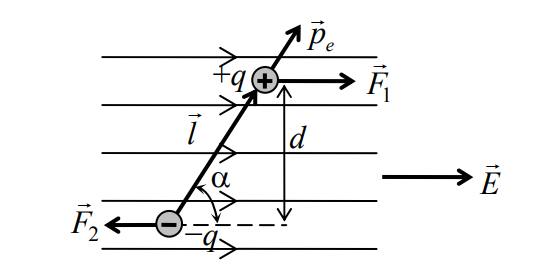
\includegraphics[]{e01_2.png}
	
	Рисунок 2
	
\end{center}

Формулу (0.5) можно записать в векторном виде:

\begin{equation}
\vec{M} = \vec{p_e} \times \vec{E}.
\end{equation}

Момент сил стремится повернуть диполь так, чтобы его электрический момент $\vec{p_e}$ установился по направлению поля.

В зависимости от характера химической связи различают 3 \textbf{механизма поляризации диэлектриков}: электронный, ионный и дипольный (ориентационный).

\textbf{Электронная поляризация} присуща всем диэлектрикам и превалирует в кристаллах с ковалентной связью. Под действием внешнего электрического поля $P$ происходит смещение электронов атома относительно его ядра (деформация его электронной оболочки) и возникают индуцированные диполи. Диэлектрические свойства индуцированных диполей относятся к числу резонансных явлений.

Электронный механизм поляризации является наименее инерционным, т.к. масса электрона значительно меньше массы частиц, участвующих в процессе поляризации. Время установления электронной поляризации составляет ≈ 10-15 с, что сравнимо с периодом световых колебаний.

\textbf{Ионная поляризация} наблюдается в ионных кристаллах и происходит в результате возникновения диполей вследствие относительного смещения (сдвига) положительных и отрицательных ионов под влиянием электрического поля. При этом имеет место также деформация электронных оболочек ионов, что порождает электронную поляризацию. Время установления ионной поляризации примерно на порядок больше ( ≈ 10-14 с).

\textbf{Дипольная (ориентационная) поляризация} наблюдается в полярных диэлектриках. Существующие в отсутствии электрического поля электрические диполи ориентированы хаотично. При включении поля диполи приобретают преимущественную ориентацию. Этот процесс и называют дипольный или ориентационной поляризацией.
\end{document}